\begin{figure}[htbp]
\centering
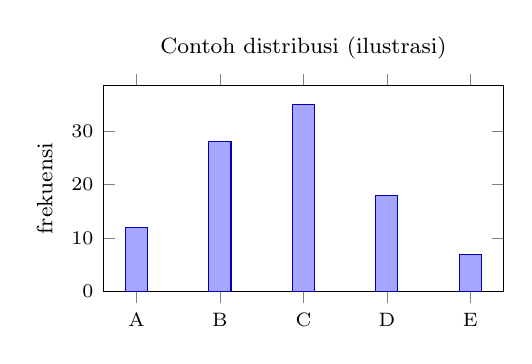
\begin{tikzpicture}
\begin{axis}[
  ybar,
  bar width=8pt,
  width=0.55\textwidth,
  height=4.2cm,
  ymin=0,
  symbolic x coords={A,B,C,D,E},
  xtick=data,
  ylabel={\footnotesize frekuensi},
  tick label style={font=\scriptsize},
  title={\footnotesize Contoh distribusi (ilustrasi)}
]
\addplot[fill=blue!35, draw=blue!70!black] coordinates {(A,12) (B,28) (C,35) (D,18) (E,7)};
\end{axis}
\end{tikzpicture}
\caption{Histogram batang ilustratif: bentuk seperti ini membantu melihat kemiringan, multimodalitas, dan ekor berat sebelum memilih transformasi atau model.}
\end{figure}
